\documentclass[11pt,a4paper]{article}
\usepackage{polski}
\usepackage[utf8]{inputenc}
\usepackage{amsthm}
\usepackage{graphicx}
\usepackage{hyperref} 

\newtheorem{twr}{Twierdzenie}


\title{Obliczanie wartości funkcji $\arctan{x}$ i $\arccot{x}$}
\author{Kamil Michalak}
\date{Analiza Numeryczna (M) - Zadanie P1.10}
\begin{document}
    \maketitle
    \section{Wstęp}
    \subsection{Treść zadania}
    Wykorzystując jedynie podstawowe działania arytmetyczne ($+$, $-$, $x$, $/$), zaproponuj efektywne sposoby wyznaczania wartości funkcji $f(x) = \arctan{x}$ i $g(x) = \arccot{x}$ z dokładnością bliską dokładności maszynowej. Opracowane algorytmy porównaj z funkcjami bibliotecznymi.
    \subsection{Sposoby rozwiązania}
    Najoczywistszym rozwiązaniem wydaje się być rozwinięcie skorzystanie z Twierdzenia funkcji w szereg. Znamy wartość tych funkcji w zerze więc możemy znaleźć szereg potęgowy tych funkcji i policzyć ich wartości wykorzystując pewną liczbą początkowych składników szeregu.
    \subsection{Dane techniczne}
    Wszystkie programy wykorzystywane w ekseperymentach zaprogramowałem w języku Julia, w wersji 1.0.1. Do obliczeń wykorzystywałem liczby zmiennoprzecinkowe o precyzji 1024 (1024 bity na mantysę). Obliczenia przeprowadziłem na komputerze z procesorem Intel Core i5 i 8 GB pamięci RAM.
    \section{Rozwinięcie funkcji w szereg Maclaurina}
    \begin{twr}[Taylora]
        Jeśli funkcja $f$ ma n pochodnych w otoczeniu punktu a,wówczas dla każdego punktu z tego otoczenia spełniony jest wzór
        \begin{displaymath}
            f(x) = f(a)+\frac{x-a}{1!}f^{(1)}(a)+\frac{(x-a)^{2}}{2!}f^{(2)}(a)+...+\frac{(x-a)^{n}}{n!}f^{(n)}(a)+R_{n+1}(x)
        \end{displaymath}
        Gdzie \begin{math} R_{n+1}(x) = \frac{f^{(n+1)}(c)}{(n+1)!}(x-a)^{(n+1)} \end{math}
    \end{twr}
    Dla a = 0 otrzymujemy szereg Maclaurina.
    \begin{displaymath}
        f(x) = f(0)+\frac{x}{1!}f^{(1)}(0)+\frac{x^{2}}{2!}f^{(2)}(0)+...+\frac{x^{n}}{n!}f^{(n)}()+R_{n+1}(x)
    \end{displaymath}
    \\\\
    \textbf{Rozwinięcie funkcji $f(x)=\arctan{x}$}      
    $$(\arccot{x})' = \frac{1}{1+x^2}$$
    Policzmy szereg Maclaurina dla funkcji $g(x)=\frac{1}{1+x^2}$. Wykorzystamy do tego funkcję $h(x)=\frac{1}{1-x}$, a następnie w miejsce $x$ wstawimy $-x^2$. \newline
    $$h'(x) = \frac{1}{(x-1)^2},\ h''(x) = -\frac{2}{(x-1)^3},\ h'''(x) = \frac{3*2}{(x-1)^4}$$\newline
    $$h^{(n)}(x) = \frac{(-1)^{n+1}n!}{(x-1)^{n+1}}$$
    Stąd
    $$h^{(n)}(0) = \frac{(-1)^{n+1}n!}{(-1)^{n+1}}=n!$$
    Szereg Maclaurina funkcji h jest więc równy
    $$\sum_{n=0}^{\infty}\frac{f^{(n)}(0)}{n!}x^{n} = \sum_{n=0}^{\infty}\frac{n!}{n!}x^{n} = \sum_{n=0}^{\infty}x^{n}$$
    Podstawiając $-x^{2}$ w miejsce $x$ otrzymujemy szereg funkcji $g(x)=\frac{1}{1+x^2}$.
    $$\frac{1}{1+x^2}=\sum_{n=0}^{\infty}(-1)^{n}x^{2n}$$
    Teraz, żeby obliczyć szereg funkcji $\arctan{x}$, posłużymy się twierdzeniem o całkowaniu szeregu potęgowego.
    \begin{twr}[O całkowaniu szeregu potęgowego]
        Niech $\sum_{n=0}^{\infty}c_nx^n$ będzie szeregiem potęgowym o promieniu zbieżności R (przy czym $0<R<\infty$) i niech S(x) oznacza sumę tego szeregu dla $x \in (-R,R)$: $S(x)=\sum_{n=0}^{\infty}c_nx^n$,\\
        Wówczas dla każdego $x \in (-R,R)$ zachodzi równość
        $$\int_0^xS(t)dt = \sum_{n=0}^{\infty}\frac{c_n}{n+1}x^{n+1},$$
        którą zapisujemy również w postaci
        $$\int_0^x(\sum_{n=0}^{\infty}c_nt^n)dt = \sum_{n=0}^{\infty}\frac{c_n}{n+1}x^{n+1}$$
    \end{twr}
    $$\arctan{x} = \int\frac{1}{1+x^2}dx + C$$
    więc $$ \int_0^x\frac{1}{1+t^2}dt = \arctan{t} |_0^x = \arctan{x}$$ % = \int\sum_{n=0}^{\infty}(-1)^{n}x^{2n} = \sum_{n=0}^{\infty}(-1)^{n}\int_{}^{}x^{2n} = \sum_{n=0}^{\infty}\frac{(-1)^{n}}{2n+1}x^{2n+1}+C$$
    %Podstawiając x=0 do równania $\arctan{x} = \sum_{n=0}^{\infty}\frac{(-1)^{n}}{2n+1}x^{2n+1}+C$ uzyskujemy $C = 0$, więc
    zatem z twierdzenia o całkowaniu szeregu potęgowego
    $$\arctan{x} = \sum_{n=0}^{\infty}\frac{(-1)^{n}}{2n+1}x^{2n+1}$$
    Ten szereg jest zbieżny dla $x\in(-1,1)$, więc umożliwi nam obliczenie wartości funkcji tylko w tym przedziale.\\
    Nie możemy liczyć kolejnych wyrazów szeregu nieskończoność, dlatego zamienimy wzór na 
    $$\arctan{x} = \sum_{n=0}^{k}\frac{(-1)^{n}}{2n+1}x^{2n+1}$$
    i sprawdzimy jego dokładność dla różnych wartości k
    \\\\
    \textbf{Rozwinięcie funkcji $g(x)=\arccot{x}$}\\\\
    Wiemy, że $\arctan{x}+\arccot{x} = \frac{\pi}{2}$, więc $\arccot{x} = \frac{\pi}{2}-\arctan{x}$.\\
    Zatem nasz wzór będzie miał postać:
    $$\arccot{x} = \frac{\pi}{2}+\sum_{n=0}^{k}\frac{(-1)^{n+1}}{2n+1}x^{2n+1}$$
    \section{Implementacja szeregu Maclaurina w Julii}
    \subsection{funkcja arctg(x)}
    Poniższy program wylicza $\arctan{x}$, wykorzystując wzór Taylora i wykonując k iteracji.
    \begin{verbatim}
        arctg_taylor(x,k)
            sum := 0
            power := x
            for i = 0,1,...,k
                if i mod 2 = 0:
                    sum := sum + power/(2*i+1)
                else
                    sum := sum - power/(2*i+1)
                power := power*x^2
            return sum
    \end{verbatim}

    Na poniższym rysunku widnieją wykresy funkcji \verb!arctg_taylor(x,50)!, oraz bibliotecznej funkcji \verb!atan(x)! wyliczającej $\arctan{x}$.\\

    \begin{figure}[h]
        \centering
        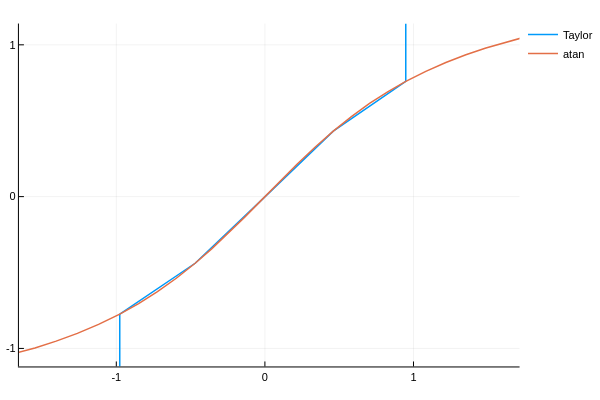
\includegraphics[width=0.9\textwidth]{arctg_taylor}
        \caption{Wykres funkcji $arctg\_taylor(x,50)$ i $atan(x)$}
    \end{figure}

    Jak można zauważyć, nasz szereg faktycznie daje w przybliżeniu dobre wyniki jedynie dla przedziału (-1,1). Widać również, że dla niektórych x nasz szereg nie jest do końca dokładny. Powinniśmy sprawdzić jak rośnie $arctg\_taylor(x,k)$ dokładność szeregu wraz ze zwiększaniem wartości k. Można to zrobić w następujący sposób - dla danego k:\\
    1. Policzyć wartość arctg-taylor(x,k) dla x=-0.99;-0.98;...;0.99.\\
    2. Dla każdej z tych wartości obliczyć błąd względny, uznając za wartość dokładną wynik funkcji bibliotecznej atan.\\
    3. Obliczyć średni błąd, ze wszystkich błędów z kroku 2.\\

    Funkcja licząca nasz średni błąd wygląda następująco

    \begin{verbatim}
        avg_error(k)
            error_sum := 0
            iterations := 0
            for i = -0.99,-0.98,...,0.99
                iterations := iterations+1
                taylor := arctg_taylor(i, k)
                arctg := atan(i)
                error_sum := error_sum + abs((x-y)/y)
            return error_sum/iterations
    \end{verbatim}

    Wyniki obliczeń prezentuje poniższa tabela.\\

    \begin{tabular}{|l|l|}
        \hline
        \textbf{k} & \textbf{Średni błąd rzędu} \\
        \hline
        5 & $10^{-3}$\\
        10 & $10^{-5}$\\
        50 & $10^{-5}$\\
        100 & $10^{-6}$\\
        500 & $10^{-9}$\\
        1000 & $10^{-15}$\\
        5000 & $10^{-50}$\\
        10000 & $10^{-94}$\\
        100000 & $10^{-308}$\\
        1000000 & $10^{-308}$\\
        \hline
    \end{tabular}\\\\\\
    Jak widać w tabeli, dla $k = 10^5$ i $k = 10^6$ uzyskaliśmy identyczny średni błąd. Oznacza, to że od pewnego momentu kolejne składniki sumy zaokroglają się do zera, nie ma więc sensu uruchamiać funkcji dla k większych od pewnego $k_0$. Doświadczalnie sprawdziłem, że $k_0 = 34700$. $10^{-308}$ to błąd rzędu precyzji arytmetyki ($2^{-1024}$)\\

    Na wykresie (1) możemy zauważyć, że dokładność naszej funkcji jest lepsza dla x bliskich 0 a gorsza na krańcach przedziału (-1,1). Ma to oczywiście sens - dla x bliskiego zeru, kolejne składniki sumy szybciej dążą do zera, więc kolejne sumy szybciej dążą do dokładnej wartości arctg(x). Warto sprawdzić jaka jest różnica w dokładności funkcji arctg\_taylor(x,k) między argumentami bliższymi i dalszymi od zera. W tym celu można przerobić funkcję avg\_error(k) tak by policzyła średni błąd dla mniejszych przedziałów.\\

    Wyniki dla k=1000\\

    \begin{tabular}{|l|l|}
        \hline
        \textbf{Przedział} & \textbf{Średni błąd rzędu}\\
        \hline
       $[0,0.2]$ & $10^{-308}$ \\
       $[0.2,0.4]$ & $10^{-308}$ \\
       $[0.4,0.6]$ & $10^{-308}$ \\
       $[0.6,0.8]$ & $10^{-199}$ \\
       $[0.8,0.99]$ & $10^{-14}$ \\
       \hline
    \end{tabular}\\\\\\
    Dla przedziałów z lewej strony zera uzyskujemy identyczne wyniki. Jak widać dokładność jest bardzo duża dla większej części przedziału ale od pewnego $x_0$ zaczyna szybko maleć (doświadczalnie sprawdziłem, że $x_0 \approx \pm 0.7$)

    \subsection{Funkcja arcctg(x)}
    W języku Julia nie ma funkcji blibliotecznej obliczającej $\arccot{x}$, można ją obliczyć za pomocą wyrażenia \verb!pi/2-atan(x)!. Wyrażenie \verb!pi/2-arctg_taylor(x,k)! oblicza $\arccot{x}$ używając tylko czterech podstawowych działań. Przeprowadzając te same eksperymenty co dla funkcji $\arctan{x}$ uzyskałem identyczne wyniki.

    \section{Obliczanie wartości funkcji poza przedziałem (-1,1)}
    Do obliczania wartości $\arctan{x}$ możemy, wykorzystać zależność, że $\arctan{x}=y \Leftrightarrow \tan{y}=x$. Jeśli będziemy potrafili obliczyć $\tan{y}$ używając jedynie 4 podstawowych działań, będziemy mogli znaleźć taki y, że $\tan{y}=x$ za pomocą metod numerycznych (np. bisekcji lub Newtona), będziemy tylko musieli je lekko zmodyfikować, tak żeby znajdowały odpowiedni y dla różnych wartości x, nie tylko dla zera.
    \subsection{Obliczanie wartości funkcji tgx}
    Wiemy, że $\tan{x}=\frac{\sin{x}}{cos{x}}$, znajdźmy więc szeregi Maclaurina dla funkcji sinus i cosinus.

    $$
        \sin{x} = \sin{0}+\frac{x}{1!}\cos{0}-\frac{x^2}{2!}\sin{0}-\frac{x^3}{3!}+\frac{x^4}{4!}\sin{0}-...
        = 0 + \frac{x}{1!}*1 - \frac{x^2}{2!}*0 - \frac{x^3}{3!}*1 + ... = \frac{x}{1!} - \frac{x}{3!} + \frac{x}{5!} - ...$$
    $$    = \sum_{n=0}^{\infty}\frac{(-1)^n}{(2n+1)!}x^{2n+1}$$\\\\

    $$ \cos{x} = \cos{0}-\frac{x}{1!}\sin{0}-\frac{x^2}{2!}\cos{0} + ... = 1 - \frac{x^2}{2!} + \frac{x^4}{4!} - ... = $$
    $$    = \sum_{n=0}^{\infty}\frac{(-1)^n}{(2n)!}x^{2n}$$

    Do obliczania wartości $\sin{x}, \cos{x}, \tg{x}$ wykorzystamy poniższe funkcje.

    \begin{verbatim}
        sin_taylor(x,k)
            sum := 0
            power := x
            fact := 1
            for i = 0,1,...,k
                if i mod 2 = 0
                    sum := sum + power/fact
                else
                    sum := sum - power/fact
                power = := power*x^2
                fact = := fact*(2*(i+1))*(2*(i+1)+1)
            return sum

        cos_taylor(x,k)
            sum := 0
            power := 1
            fact := 1
            for i = 0,1,...,k
                if i mod 2 = 0
                    sum := sum + power/fact
                else
                    sum := sum - power/fact
                power = := power*x^2
                fact = := fact*(2*(i+1)-1)*(2*(i+1))
            return sum

        tg_taylor(x,k)
            if x = 0 return 0
            else return sin_taylor(x,k)/cos_taylor(x,k)
    \end{verbatim}

    Funkcja \verb!tg_taylor(x,k)! ma największą dokładność (rzędu $10^{-305}$), dla k=200. Zwiększanie k powyżej tej wartości nie poprawia dokładności funkcji.
    
    \subsection{Wykorzystanie metody bisekcji do obliczania wartość arctgx}

    Zmodyfikowana wersja algorytmu bisekcji, znajdująca argument o wartości y, dla funkcji f, na przedziale [a,b], z zadaną dokładnością.

    \begin{verbatim}
        bisect(f,y,a,b, epsilon)
            while (abs(a-b)>epsilon)
                s := (a+q)/2.0
                if abs(f(s)-y) <= epsilon
                    break
                else if (f(s)-y) * (f(a)-y) < 0
                    b := s 
                else
                    a := s
                end
            return (a+q)/2
    \end{verbatim}
    Funkcję obliczającą $\arctan{x}$ możemy zapisać następująco (dla zadanych $k \in N$ i $epsilon > 0$).
    \begin{verbatim}
        tg(x) = tg_taylor(x,k)
        arctg(x) = bisect(tg,x,-pi/2,pi/2,epsilon)
    \end{verbatim}

    Wykres funkcji \verb!arctgx(x)!, dla $k=100$ i $epsilon=10^{-16}$, i bibliotecznej funkcji \verb!atan(x)! wygląda następująco. Różnice są na tyle małe, że nie widać ich na wykresie.\\

    \begin{figure}[h]
        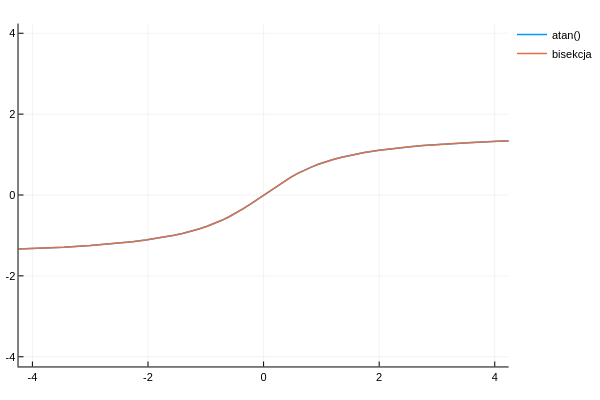
\includegraphics[width=0.9\textwidth]{bisect.png}
        \caption{Wykres funkcji $arctg(x)$ i $atan(x)$}
    \end{figure}


    Dla $k=200$ i $\epsilon=2^{-1023}$ (błąd rzędu precyzji arytmetyki) funkcja bisekcji wykonuje się ok. 2,16 s.


    \subsection{Funkcja arcctgx}
    Przy obliczaniu funkcji $\arccot{x}$ skorzystamy z faktu, że $\cot{x} = \frac{\cos{x}}{\sin{x}}$. Więc funkcja licząca $\cot{x}$ ze wzoru Taylora wygląda następująco.

    \begin{verbatim}
    ctg_taylor(x,k)
            if x = pi/2 return 0
            else return cos_taylor(x,k)/sin_taylor(x,k)
    \end{verbatim}

    Identycznie jak dla funkcji \verb!tg_taylor(x,k)!, dokładność funkcji \verb!ctg_taylor(x,k)! jest największa dla $k=200$ i nie poprawia się dla większych k.\\
    Możemy z jej pomocą policzyć $\arccot{x}$.
    \begin{verbatim}
        ctg(x) = tg_taylor(x,k)
        arcctg(x) = bisect(ctg,x,0,pi,epsilon)
    \end{verbatim}

    Wykres funkcji \verb!arctgx(x)!, dla $k=100$ i $epsilon=10^{-16}$, i  funkcji \verb!pi/2 - atan(x)!:
    \begin{figure}[h]
        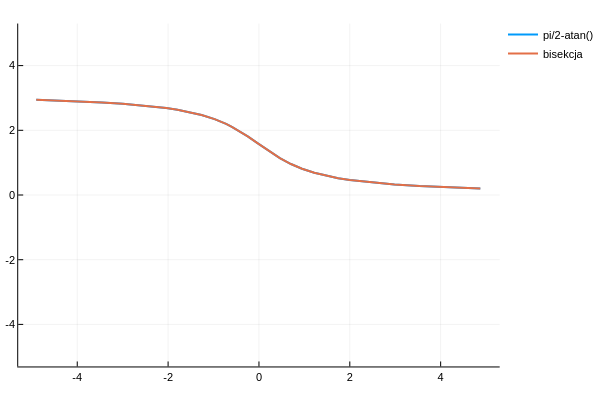
\includegraphics[width=0.9\textwidth]{bisect2.png}
        \caption{Wykres funkcji $arcctg(x)$ i $pi/2-atan(x)$}
    \end{figure}

    \section{Wnioski}
    Wartości $\arctan{x}$ i $\arccot{x}$ dla $x\in(-1,1)$ najlepiej liczyć ze wzoru Taylora. Dla liczb spoza tego przedziału trzeba korzystać z innych metod. Metoda zaprezentowana przeze mnie - wykorzystująca bisekcję na funkcji $\tan{y}$/$\cot{y}$ do znalezienia argumentu o wartości równej $\arctan{x}$/$\arccot{x}$ nie jest szczególnie szybka ale umożliwia obliczenie szukanej wartości z dużą dokładnością. Nadaje się do obliczania wartości funkcji dla niewielkiej liczby argumentów.

    \section{Źródła}
    \begin{itemize}
        \item \href{http://prac.im.pwr.wroc.pl/~kajetano/AM2/}{http://prac.im.pwr.wroc.pl/~kajetano/AM2/}
    \end{itemize}
        
\end{document}